\documentclass[compress,red]{beamer}
\usepackage[utf8]{inputenc}
\usepackage{ucs}
\usepackage{amsmath}
\usepackage{amsfonts}
\usepackage{amssymb}
\usepackage[russian]{babel}
\usepackage{graphicx}
\usepackage{wrapfig}

\usepackage{tikz}
\usepackage{verbatim}

\usepackage{color}
\usepackage{xcolor}
\usepackage{listings}

\usepackage{caption}
\DeclareCaptionFont{white}{\color{white}}
\DeclareCaptionFormat{listing}{\colorbox{gray}{\parbox{\textwidth}{#1#2#3}}}
\captionsetup[lstlisting]{format=listing,labelfont=white,textfont=white}

\usetikzlibrary{calc,trees,positioning,arrows,chains,shapes.geometric,%
    decorations.pathreplacing,decorations.pathmorphing,shapes,%
    matrix,shapes.symbols}

\tikzset{
>=stealth',
  punktchain/.style={
    rectangle, 
    rounded corners, 
    % fill=black!10,
    draw=black, very thick,
    text width=10em, 
    minimum height=3em, 
    text centered, 
    on chain},
  line/.style={draw, thick, <-},
  element/.style={
    tape,
    top color=white,
    bottom color=blue!50!black!60!,
    minimum width=8em,
    draw=blue!40!black!90, very thick,
    text width=10em, 
    minimum height=1.5em, 
    text centered, 
    on chain},
  every join/.style={->, thick,shorten <=1pt},
  decoration={brace},
  tuborg/.style={decorate},
  tubnode/.style={midway, right=2pt},
}

\mode<presentation>

\usetheme{Warsaw}

\definecolor{Red}{rgb}{1,0,0}
\definecolor{Blue}{rgb}{0,0,1}
\definecolor{Green}{rgb}{0,1,0}
\definecolor{magenta}{rgb}{1,0,.6}
\definecolor{lightblue}{rgb}{0,.5,1}
\definecolor{lightpurple}{rgb}{.6,.4,1}
\definecolor{gold}{rgb}{.6,.5,0}
\definecolor{orange}{rgb}{1,0.4,0}
\definecolor{hotpink}{rgb}{1,0,0.5}
\definecolor{newcolor2}{rgb}{.5,.3,.5}
\definecolor{newcolor}{rgb}{0,.3,1}
\definecolor{newcolor3}{rgb}{1,0,.35}
\definecolor{darkgreen1}{rgb}{0, .35, 0}
\definecolor{darkgreen}{rgb}{0, .6, 0}
\definecolor{darkred}{rgb}{.75,0,0}

\xdefinecolor{olive}{cmyk}{0.64,0,0.95,0.4}
\xdefinecolor{purpleish}{cmyk}{0.75,0.75,0,0}

\useoutertheme[subsection=false]{smoothbars}


\title{Объектно--ориентированное программирование}
\author{Информатика \\ 10-11 классы}

%\usecolortheme{dolphin}


\begin{document}
%%титульная страница
\maketitle
%% основные моменты

\section{Что такое ООП}

\subsection{Что такое ООП}
\begin{frame}
  \frametitle{Что такое ООП?}
  \begin{itemize}
    \item Динамическое и функциональное виды программирования, как известно, решают весьма важную задачу разделения \emph{бизнес--логики} приложения от низкоуровневых алгоритмов.
    \item Когда мы используем автомобиль, мы не задумываемся о его устройстве, а просто используем различные способы управления.
    \item При этом даже те инженеры, которые разрабатывают автомобили, имеют свои специализации: часть занимается двигателем, часть --- дизайном, часть --- безопасностью, а кто-то --- и концепцией в целом.
  \end{itemize}
\end{frame}

\subsection{Что такое ООП 2}
\begin{frame}
  \frametitle{Что такое ООП?}
  \begin{itemize}
    \item Концепция \emph{объектно--ориентированного программирования} (ООП) предлагает оперировать в программе не переменными и функциями, а \emph{объектами}.
    \item Всё в программе является объектами.
    \item У объекта имеются свойства и методы. 
    \item Свойства представляют собой переменные, принадлежащие объекту.
    \item Методы --- функции, позволяющие получить / изменить информацию об объекте.
  \end{itemize}
\end{frame}

\section{Кот}

\subsection{Кот}
\begin{frame}
  \frametitle{Объект Кот}
	\centerline{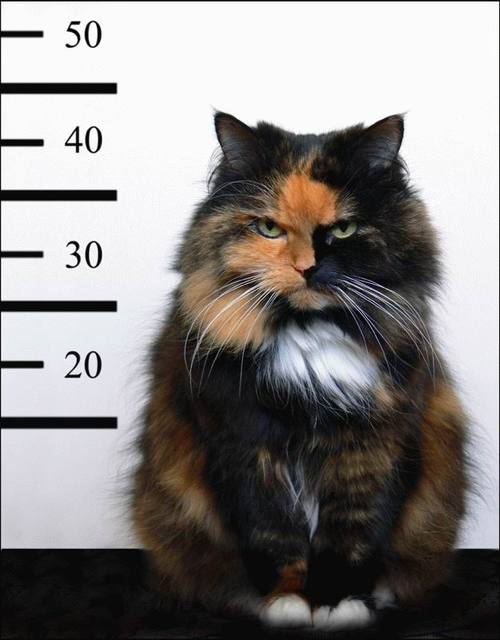
\includegraphics[width=0.5\textwidth]{images/catE.jpg}}
\end{frame}

\subsection{Свойства кота}
\begin{frame}
  \begin{center}
    \Huge{Какие свойства есть у кота?}
  \end{center}
\end{frame}

\subsection{Свойства кота список}
\begin{frame}[fragile]
  \frametitle{Свойства кота}
  \begin{itemize}
    \item Порода
    \item Цвет
    \item Рост
    \item Возраст
    \item Дата последнего кормления
    \item Дата последнего поглаживания
    \item Дата последнего мяукания
    \item ...
  \end{itemize}
\end{frame}

\subsection{Методы кота}
\begin{frame}
  \begin{center}
    \Huge{А методы?}
  \end{center}
\end{frame}

\subsection{Методы кота 2}
\begin{frame}[fragile]
  \frametitle{Методы кота}
  \begin{itemize}
    \item Мяукнуть
    \item Поесть
    \item Потребовать погладить
    \item Погулять
    \item ...
  \end{itemize}
\end{frame}

\section{Другие животные}

\subsection{Другие жывотные}
\begin{frame}
  \begin{center}
    \Huge{А что с другими животными?}
  \end{center}
\end{frame}

\subsection{Лошадко}
\begin{frame}[fragile]
  \frametitle{Упс, не то}
  \centerline{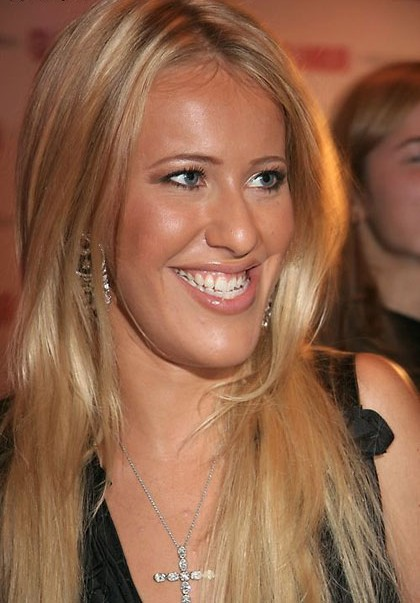
\includegraphics[width=0.4\textwidth]{images/loshadko.jpg}}
\end{frame}

\subsection{Собачка}
\begin{frame}[fragile]
  \frametitle{Собака}
  \centerline{
\includegraphics[width=0.7\textwidth]{images/dog.jpg}}
\end{frame}

\subsection{Собака}
\begin{frame}[fragile]
  \frametitle{Сравнение свойств Кота и Собаки}
  \begin{columns}[ll]
    \column{2.0in}
      \begin{itemize}
        \item Порода
        \item Цвет
        \item Рост
        \item Возраст
        \item Дата последнего кормления
        \item Дата последнего поглаживания
        \item \textbf{Дата последнего мяукания}      
      \end{itemize}
    \column{2.0in}
      \begin{itemize}
        \item Порода
        \item Цвет
        \item Рост
        \item Возраст
        \item Дата последнего кормления
        \item Дата последнего поглаживания
        \item \textbf{Дата последнего гавкания}      
      \end{itemize}
  \end{columns}
\end{frame}

\subsection{Методы собаки и кота}
\begin{frame}[fragile]
  \frametitle{Сравнение методов Кота и Собаки}
  \begin{columns}[ll]
    \column{2.0in}
      \begin{itemize}
        \item \textbf{Мяукнуть}
        \item Поесть
        \item Потребовать погладить
        \item Погулять
      \end{itemize}
    \column{2.0in}
    \begin{itemize}
      \item \textbf{Гавкнуть}
      \item Поесть
      \item Потребовать погладить
      \item Погулять
      \item \textbf{Выгуляться}
    \end{itemize}
  \end{columns}
\end{frame}

\subsection{Домашние животные}
\begin{frame}[fragile]
  \frametitle{Домашние животные}
  \centerline{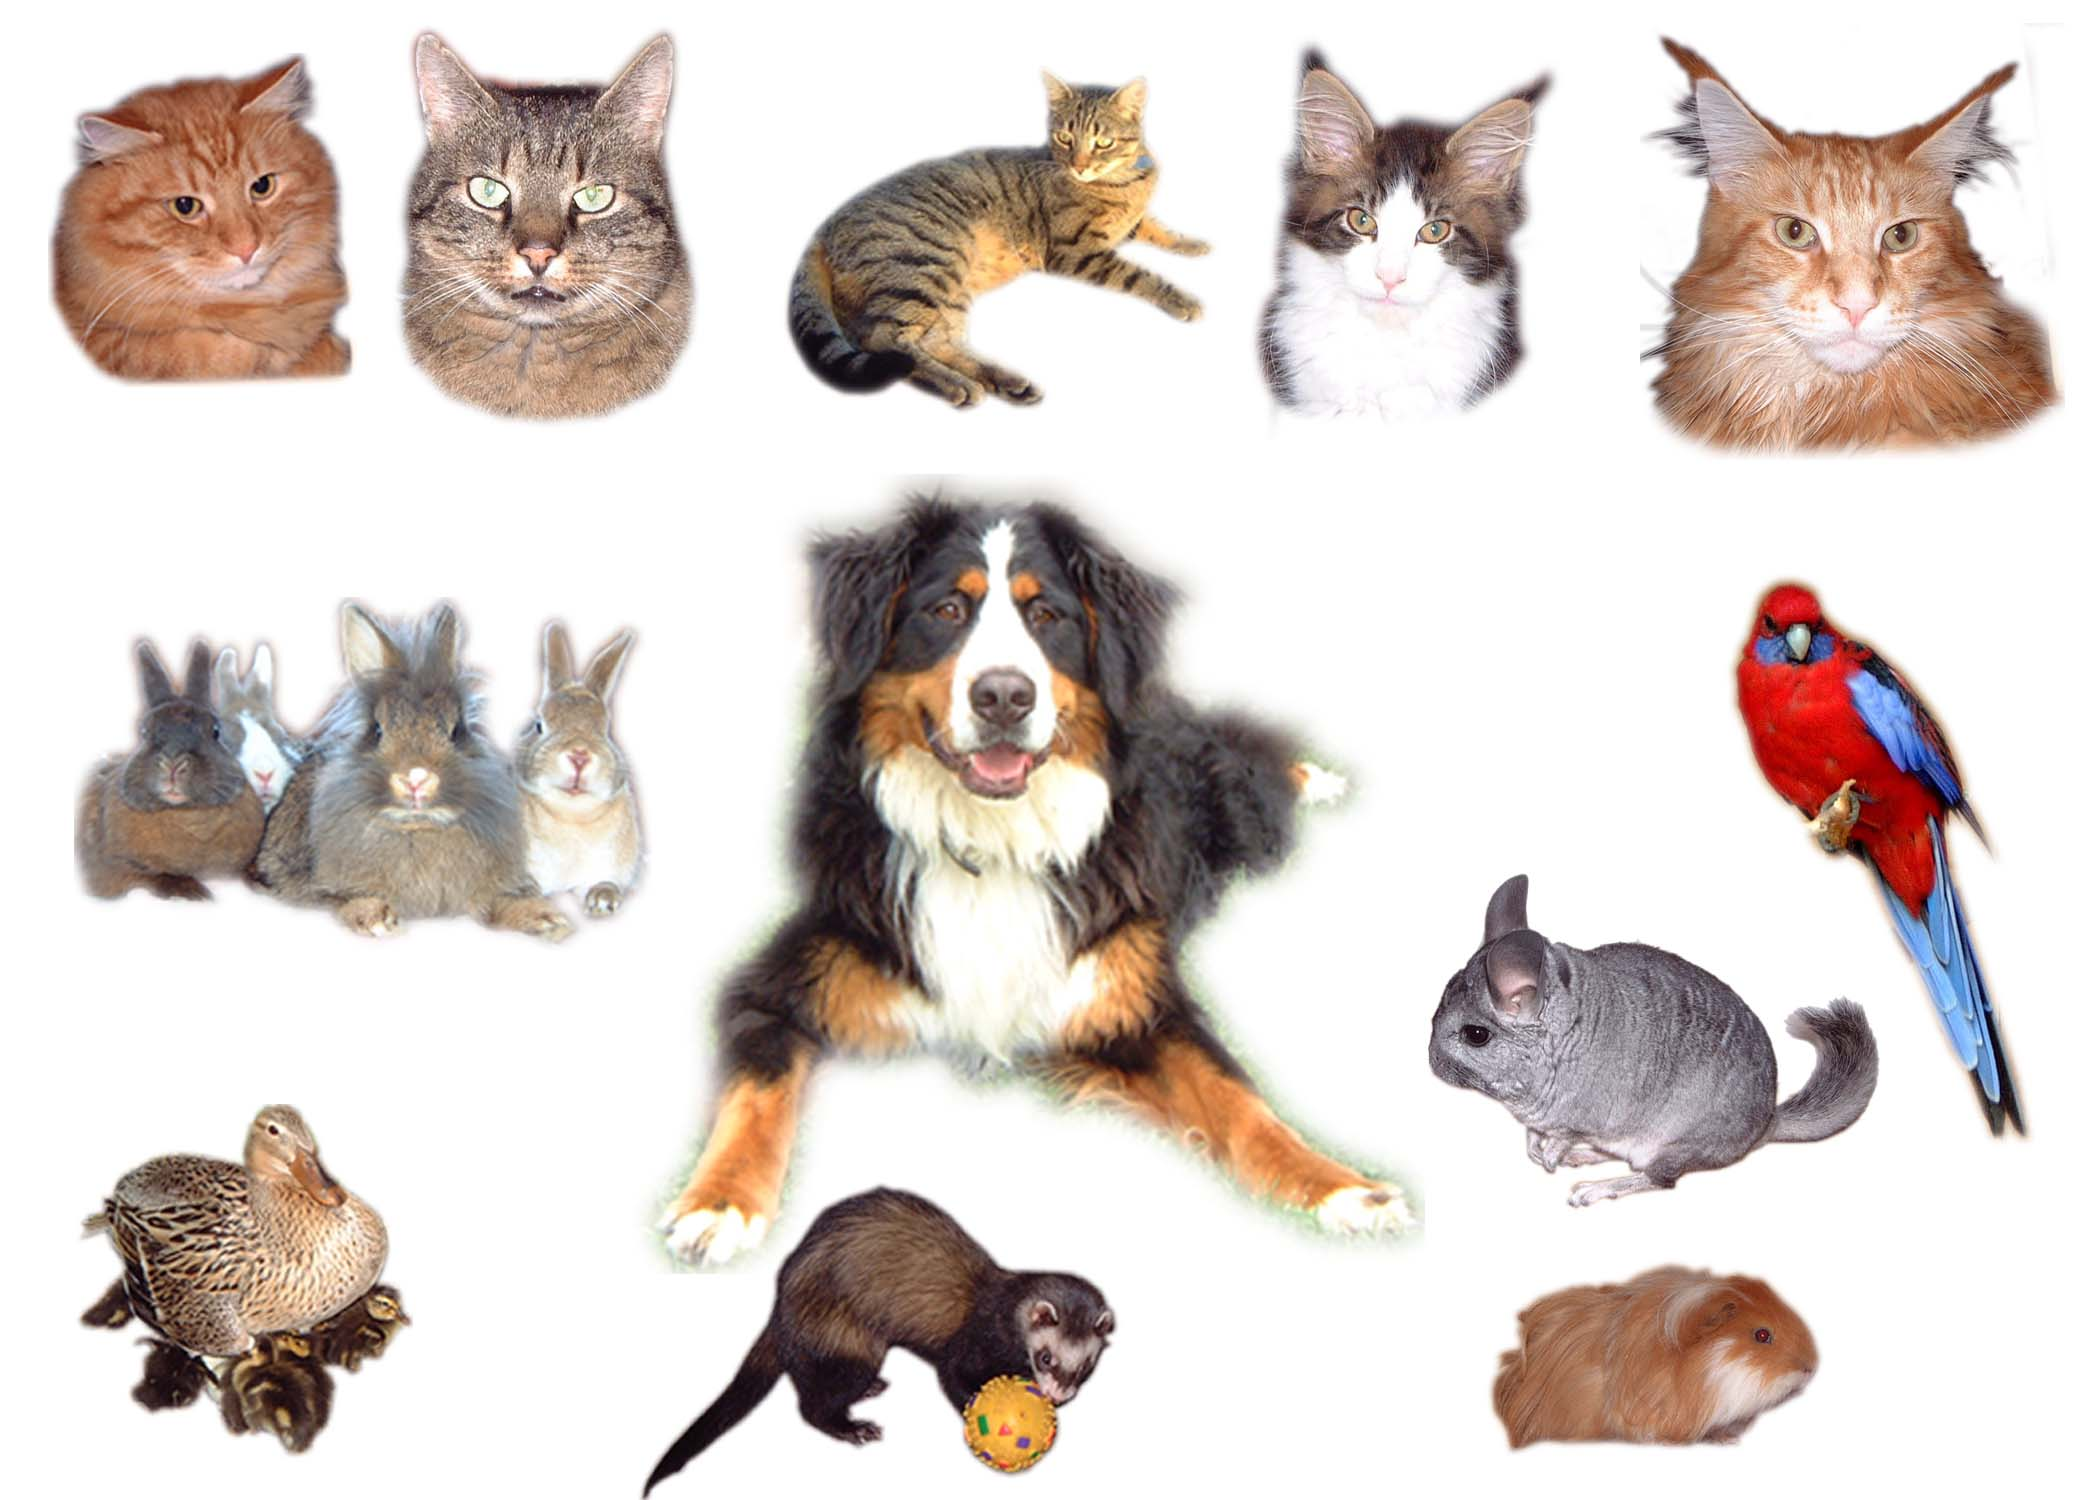
\includegraphics[width=0.7\textwidth]{images/home_animals.jpg}}
\end{frame}

\section{Наследование}
\subsection{Наследование}
\begin{frame}
  \begin{center}
    \Huge{Принцип наследования}
  \end{center}
  \begin{center}
    \Large{Общие свойства и методы объектов можно вынести в класс--\textbf{родитель}. Все ``дети''--наследники автоматически получают их.}
  \end{center}
\end{frame}

\subsection{Наследование схема}
\begin{frame}[fragile]
  \frametitle{Схема наследования}
    \begin{figure}
    \centering
    \begin{tikzpicture}[node distance=1cm, auto]  
    \tikzset{
        action/.style={rectangle,draw=black, top color=white, bottom color=yellow!50,very thick, inner sep=0.25em, minimum size=0.6em, text centered},
        input/.style={ellipse,draw=black, top color=white, bottom color=yellow!50,very thick, inner sep=0.25em, minimum size=0.6em, text centered},
        condition/.style={diamond,draw=black, top color=white, bottom color=yellow!50,very thick, inner sep=0.25em, minimum size=0.6em, text centered},
        myarrow/.style={draw},
    }
    \node[action] (item1) {Родитель: Домашнее животное};  
    \node (AuxNode01) [text width=0cm, below=3em of item1] {};
    \node[action, left=5em of AuxNode01] (item2) {Наследник: Кот};
    \node[action, right=5em of AuxNode01] (item3) {Наследник: Собака};

    \path[myarrow] (item1) -- (AuxNode01);   
    \path[myarrow] (AuxNode01) -- (item2);   
    \path[myarrow] (AuxNode01) -- (item3);   

    \end{tikzpicture} 
    \end{figure}
  
\end{frame}

\subsection{Термины}
\begin{frame}[fragile]
  \frametitle{Несколько нудных терминов}
  \begin{itemize}
    \item Одинаковые объекты являются \textbf{экземплярами класса}.
    \item Кот --- это, на самом деле, класс.
    \item А вот, например, кот Вася --- это объект, то есть, представитель класса.
    \item Класс --- это программная структура. 
    \item В программе мы сначала создаём класс, а потом уже создаём (\textbf{инстанцируем}) объекты.
    \item В ruby всё что угодно является объектом. Даже число 5, строка ``мама мыла раму'' и пр.
  \end{itemize}
\end{frame}

\section{Примеры}
\subsection{Примеры}
\begin{frame}[fragile]
  \frametitle{Класс Многоугольник}
  \begin{itemize}
    \item Создадим класс Многоугольник.
    \item Базовые свойства фигуры: стороны фигуры, углы, периметр, площадь и др.
    \item Методы: посчитать площадь, посчитать периметр, найти радиус описанной окружности и др.
    \item Фигуры бывают разные: треугольник, четырёхугольник (среди которых тоже есть квадрат, ромб и пр.)
    \item У каких-то фигур мы знаем, как считать площадь и пр., а у каких-то --- нет.
    \item Напишем программу.
  \end{itemize}
\end{frame}

\subsection{Класс Многоугольник}
\begin{frame}[fragile]
  \frametitle{Класс Многоугольник}
  \scriptsize{
  \begin{lstlisting}[language=ruby,basicstyle=\footnotesize,label=ruby1,caption=Класс Многоугольник]
    class Polygon
      attr_accessor :sides, :corners,
                    :perimeter, :square
      def perimeter
        @perimeter = @sides.inject(0){|res, elem| 
                                      res + elem}
      end
      def num_points
        @sides.size
      end
    end
  \end{lstlisting}
  }
\end{frame}

\subsection{Разбор класса Многоугольник}
\begin{frame}[fragile]
  \frametitle{Пояснения к классу}
  \begin{itemize}
    \item Методы класса определяются точно так же, как и обычные функции. Отличий нет.
    \item Свойства класса мы будем определять через специальную конструкцию \textbf{attr\_accessor}. Не вдаваясь в детали, просто перечислим все свойства--переменные. Обратите внимание, что они начинаются со знака ``двоеточие''.
    \item Чтобы внутри метода обратиться к свойству, нужно перед его (свойства) названием поставить знак @.
    \item В данном классе мы определяем методы perimeter и num\_points (количество вершин). Мы специально метод perimeter назвали одинаково со свойством, чтобы при вызове obj.perimeter происходило автоматическое вычисление.
  \end{itemize}
\end{frame}

\subsection{Использование класса}
\begin{frame}[fragile]
  \frametitle{Используем класс Polygon}
  \scriptsize{
  \begin{lstlisting}[language=ruby,basicstyle=\footnotesize,label=ruby2,caption=Использование Polygon]
    fig = Polygon.new
    fig.sides = [2,4,2,4]
    fig.corners = [90, 90, 90, 90]

    puts fig.perimeter
  \end{lstlisting}
  }
  \begin{itemize}
    \item Для создания экземпляра класса используется конструкция CLASS.new. Аналог --- ручное создание массивов и хэшей.
    \item Некоторые свойства мы задаём вручную.
    \item Также, как и массивами, для вызова методов и свойств используем разделитель--точку.
  \end{itemize}
\end{frame}

\subsection{Наследование}
\begin{frame}[fragile]
  \frametitle{Класс Triangle}
  \scriptsize{
  \begin{lstlisting}[language=ruby,basicstyle=\footnotesize,label=ruby3,caption=Класс Triangle]
    class Triangle < Polygon
      def square
        pp = self.perimeter/2
        (pp*(pp - sides[0])*(pp-sides[1])*
        (pp-sides[2]))**0.5
      end
    end
    tr = Triangle.new
    tr.sides = [3,4,5]
    puts tr.square
    puts tr.perimeter
  \end{lstlisting}
  }
\end{frame}

\subsection{Наследование 2}
\begin{frame}[fragile]
  \frametitle{Разбор класса Triangle}
  \begin{itemize}
    \item Аналогично создаём класс Triangle, являющийся наследником класса Polygon.
    \item Для наследования используем конструкцию: Наследник < Родитель.
    \item Все методы и свойства класса Polygon автоматически появились в классе Triangle.
    \item Отдельно определяем по формуле Герона площадь треугольника.
    \item Итого, теперь в треугольнике мы можем посчитать и площадь, и периметр.
  \end{itemize}
\end{frame}

\subsection{Наследование 3}
\begin{frame}[fragile]
  \frametitle{Разбор класса Triangle}
  \begin{itemize}
    \item Разберёмся в конструкции self.perimeter.
    \item \textbf{self} означает текущий объект, то есть тот объект, для которого вызывается метод или свойство.
    \item \textbf{self.sides} --- замена \textbf{@sides}.
    \item Однако вызвать метод со знаком @ не получится. Для этого и используем конструкцию self.
    \item self.perimeter вызывает метод perimeter для текущего объекта.
    \item \textbf{Задание}. В чём отличие записи @perimeter от self.perimeter? Одинаков ли будет результат. Если нет, приведите пример.
  \end{itemize}
\end{frame}

\section{Задания}
\subsection{Задания}
\begin{frame}[fragile]
  \frametitle{Задания}
  \begin{itemize}
    \item Написать класс Прямоугольник --- наследник Polygon. Определить в нём метод подсчёта площади. Проверить корректность его работы.
    \item Написать в классе Прямоугольник метод, определяющий, является ли прямоугольник квадратом. Метод должен возвращать булевский ответ. Проверить корректность работы метода.
    \item Создать в классе Треугольник метод, проверяющий, является ли данный треугольник прямоугольным. Проверить корректность работы метода.
  \end{itemize}
\end{frame}

\section{References}
\subsection{References}
\begin{frame}[fragile]
  \frametitle{References}
  \begin{itemize}
    \item При подготовке данного материала использовались сайты: http://ru.wikibooks.org/wiki/Ruby, http://rubydev.ru, http://en.wikipedia.org, http://ruby-lang.org, http://de.trinixy.ru/, http://www.krassotkam.ru/, http://gen.su/.
    \item Все презентации доступны на http://school.smirik.ru!
    \item Вопросы, предложения, д/з: smirik@gmail.com
  \end{itemize}
\end{frame}

\end{document}